\documentclass{beamer}

\usetheme{avad}

\usepackage[utf8]{inputenc}
\usepackage{amsmath,amssymb}
\usepackage{tikz}

\newcommand{\haltpagenumber}{\addtocounter{framenumber}{-1}}

%\graphicspath{%
%{figs/}%
%}



%%%%%%%%%%%%%%%%%%%%%%%%%%%%%%%%%%%%%%%%%%%%%%%%%%%%%%%%%%%%%%%%%%%%%%%%%%%%%%%%
%%%%%%%%%%%%%%%%%%%%%%%%%%%%%%%%%%%%%%%%%%%%%%%%%%%%%%%%%%%%%%%%%%%%%%%%%%%%%%%%
\begin{document}

%%%%%%%%%%%%%%%%%%%%%%%%%%%%%%%%%%%%%%%%%%%%%%%%%%%%%%%%%%%%%%%%%%%%%%%%%%%%%%%%
\title{\centering Open Science in the Two!Ears Project \\ Experiences and Best Practices}
\author{Hagen Wierstorf$\,$\inst{1} \and
        Fiete Winter\inst{2} \and
        \textbf{Sascha Spors}\inst{2}}
        \institute{\inst{1} Centre for Vision, Speech and Signal Processing, University of Surrey\\
           \inst{2} Institute of Communications Engineering, University of Rostock}
\date{26/06/2017}
\maketitle

%%%%%%%%%%%%%%%%%%%%%%%%%%%%%%%%%%%%%%%%%%%%%%%%%%%%%%%%%%%%%%%%%%%%%%%%%%%%%%%%
\begin{frame}{Two!Ears}

    \centering
    \vspace{0.5cm}
    \textbf{Computational framework for modelling active exploratory
    listening that assigns meaning to auditory scenes}

    \vspace{1.0cm}

    \begin{minipage}[b]{0.42\columnwidth}
        \resizebox{\textwidth}{!}{%
            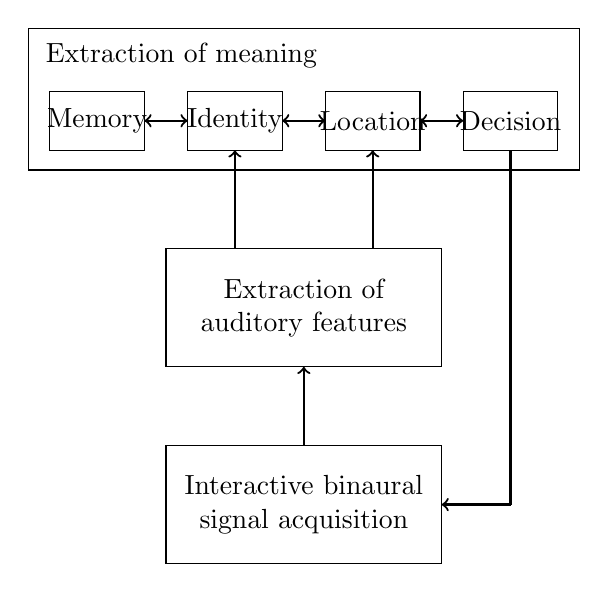
\begin{tikzpicture}
                \draw (-1.75,0) rectangle (1.75,1.5); % binaural simulator
                \node[align=center] at (0,0.75) {Interactive binaural\\ signal acquisition};
                \draw (-1.75,2.5) rectangle (1.75,4); % auditory front-end
                \node[align=center] at (0,3.25) {Extraction of\\ auditory features};
                \draw (-3.5,5) rectangle (3.5,6.8); % blackboard
                \node[right] at (-3.4,6.45) {Extraction of meaning};
                \draw (-3.225,5.25) rectangle (-2.025,6);
                \node at (-2.625,5.625) {\ft Memory};
                \draw (-1.475,5.25) rectangle (-0.275,6);
                \node at (-0.875,5.625) {\ft Identity};
                \draw ( 0.275,5.25) rectangle ( 1.475,6);
                \node at (0.875,5.625) {\ft Location};
                \draw ( 2.025,5.25) rectangle ( 3.225,6);
                \node at (2.625,5.625) {\ft Decision};
                \draw[thick,->] (0,1.5) -- (0,2.5);
                \draw[thick,->] (-0.875,4) -- (-0.875,5.25);
                \draw[thick,->] ( 0.875,4) -- ( 0.875,5.25);
                \draw[thick] (2.625,5.25) -- (2.625,0.75);
                \draw[thick,->] (2.625,0.75) -- (1.75,0.75);
                \draw[thick,<->] (-2.025,5.625) -- (-1.475,5.625);
                \draw[thick,<->] (-0.275,5.625) -- ( 0.275,5.625);
                \draw[thick,<->] ( 1.475,5.625) -- ( 2.025,5.625);
            \end{tikzpicture}
        }
    \end{minipage}
    \hfill
    \begin{minipage}[b]{.54\columnwidth}
        \begin{itemize}
            \item 9 international partners
            \item Test single components
            \item Allow for feedback
            \item Dynamic input signals
        \end{itemize}
        $\Rightarrow$ \textbf{common software} \\
        $\Rightarrow$ \textbf{common data}

        \vspace{1cm}

    \end{minipage}

\end{frame}

%%%%%%%%%%%%%%%%%%%%%%%%%%%%%%%%%%%%%%%%%%%%%%%%%%%%%%%%%%%%%%%%%%%%%%%%%%%%%%%%
\begin{frame}{Open Science}

    Goal of Two!Ears: follow Open Science approach

    \vspace{0.5cm}

    \begin{itemize}
        \item Open source
        \item Open data
        \item Open access
    \end{itemize}

\end{frame}

%%%%%%%%%%%%%%%%%%%%%%%%%%%%%%%%%%%%%%%%%%%%%%%%%%%%%%%%%%%%%%%%%%%%%%%%%%%%%%%%
\begin{frame}{Comparison with AMToolbox}

    \vspace{0.3cm}

    Auditory Modeling Toolbox
    \vspace{0.1cm}
    \begin{itemize}
        \item AABBA project started in 2009: \textbf{apply binaural models}
        \item Model source code rarely available
        \item Initiated open collection of models: \\
            {\small\url{http://amtoolbox.sourceforge.net}}
    \end{itemize}

    \vspace{0.6cm}

    Additional required features by Two!Ears
    \vspace{0.1cm}
    \begin{itemize}
        \item Block-based processing
        \item Clear separation in feature extraction and machine learning
        \item Easy combination of different models
        \item Initiated dedicated modeling approach: \\
            {\small\url{http://docs.twoears.eu}}
    \end{itemize}

\end{frame}

%%%%%%%%%%%%%%%%%%%%%%%%%%%%%%%%%%%%%%%%%%%%%%%%%%%%%%%%%%%%%%%%%%%%%%%%%%%%%%%%
\begin{frame}{Two!Ears auditory model}

    \vspace{1cm}

    \begin{minipage}[b]{0.42\columnwidth}
        \resizebox{\textwidth}{!}{%
            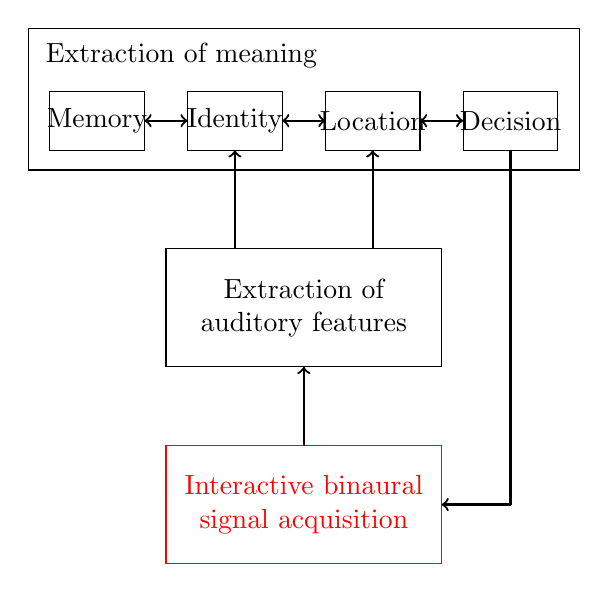
\begin{tikzpicture}
                \draw[color=red] (-1.75,0) rectangle (1.75,1.5); % binaural simulator
                \node[align=center,color=red] at (0,0.75) {Interactive binaural\\ signal acquisition};
                \draw (-1.75,2.5) rectangle (1.75,4); % auditory front-end
                \node[align=center] at (0,3.25) {Extraction of\\ auditory features};
                \draw (-3.5,5) rectangle (3.5,6.8); % blackboard
                \node[right] at (-3.4,6.45) {Extraction of meaning};
                \draw (-3.225,5.25) rectangle (-2.025,6);
                \node at (-2.625,5.625) {\ft Memory};
                \draw (-1.475,5.25) rectangle (-0.275,6);
                \node at (-0.875,5.625) {\ft Identity};
                \draw ( 0.275,5.25) rectangle ( 1.475,6);
                \node at (0.875,5.625) {\ft Location};
                \draw ( 2.025,5.25) rectangle ( 3.225,6);
                \node at (2.625,5.625) {\ft Decision};
                \draw[thick,->] (0,1.5) -- (0,2.5);
                \draw[thick,->] (-0.875,4) -- (-0.875,5.25);
                \draw[thick,->] ( 0.875,4) -- ( 0.875,5.25);
                \draw[thick] (2.625,5.25) -- (2.625,0.75);
                \draw[thick,->] (2.625,0.75) -- (1.75,0.75);
                \draw[thick,<->] (-2.025,5.625) -- (-1.475,5.625);
                \draw[thick,<->] (-0.275,5.625) -- ( 0.275,5.625);
                \draw[thick,<->] ( 1.475,5.625) -- ( 2.025,5.625);
            \end{tikzpicture}
        }
    \end{minipage}
    \hfill
    \begin{minipage}[b]{0.56\columnwidth}

        \centering
        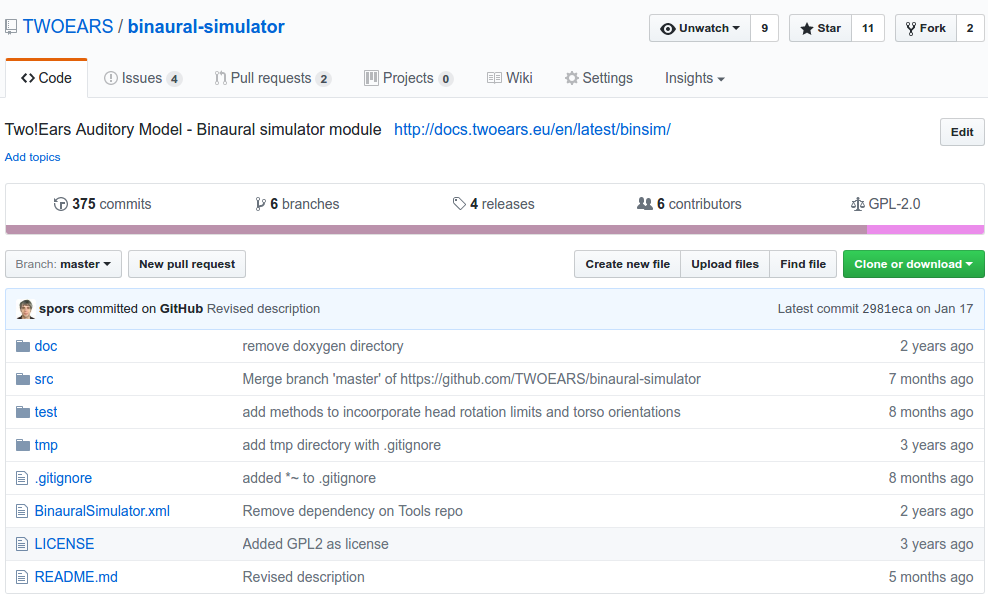
\includegraphics[width=.9\textwidth]{fig/binaural-simulator}

        \begin{itemize}
            \item Standalone ready
            \item Defined interface to other modules
        \end{itemize}

    \end{minipage}

\end{frame}

%%%%%%%%%%%%%%%%%%%%%%%%%%%%%%%%%%%%%%%%%%%%%%%%%%%%%%%%%%%%%%%%%%%%%%%%%%%%%%%%
\begin{frame}{Two!Ears auditory model}

    \haltpagenumber

    \vspace{1cm}

    \begin{minipage}[b]{0.42\columnwidth}
        \resizebox{\textwidth}{!}{%
            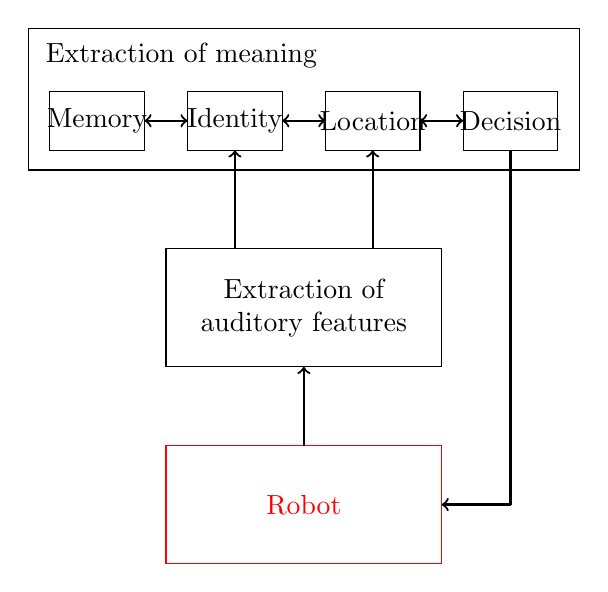
\begin{tikzpicture}
                \draw[color=red] (-1.75,0) rectangle (1.75,1.5); % binaural simulator
                \node[align=center,color=red] at (0,0.75) {Robot};
                \draw (-1.75,2.5) rectangle (1.75,4); % auditory front-end
                \node[align=center] at (0,3.25) {Extraction of\\ auditory features};
                \draw (-3.5,5) rectangle (3.5,6.8); % blackboard
                \node[right] at (-3.4,6.45) {Extraction of meaning};
                \draw (-3.225,5.25) rectangle (-2.025,6);
                \node at (-2.625,5.625) {\ft Memory};
                \draw (-1.475,5.25) rectangle (-0.275,6);
                \node at (-0.875,5.625) {\ft Identity};
                \draw ( 0.275,5.25) rectangle ( 1.475,6);
                \node at (0.875,5.625) {\ft Location};
                \draw ( 2.025,5.25) rectangle ( 3.225,6);
                \node at (2.625,5.625) {\ft Decision};
                \draw[thick,->] (0,1.5) -- (0,2.5);
                \draw[thick,->] (-0.875,4) -- (-0.875,5.25);
                \draw[thick,->] ( 0.875,4) -- ( 0.875,5.25);
                \draw[thick] (2.625,5.25) -- (2.625,0.75);
                \draw[thick,->] (2.625,0.75) -- (1.75,0.75);
                \draw[thick,<->] (-2.025,5.625) -- (-1.475,5.625);
                \draw[thick,<->] (-0.275,5.625) -- ( 0.275,5.625);
                \draw[thick,<->] ( 1.475,5.625) -- ( 2.025,5.625);
            \end{tikzpicture}
        }
    \end{minipage}
    \hfill
    \begin{minipage}[b]{0.56\columnwidth}

        \centering
        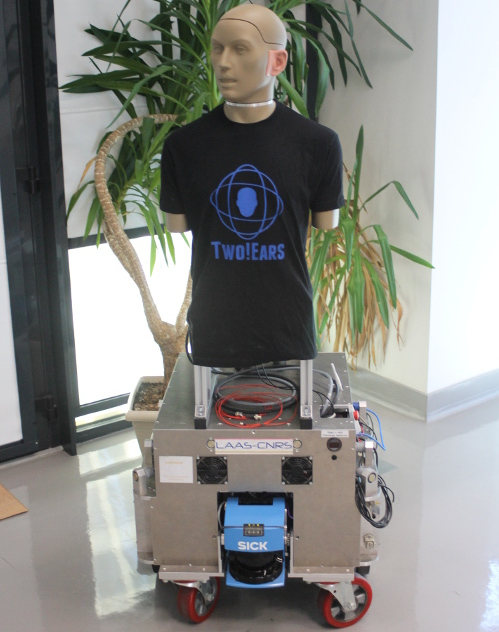
\includegraphics[width=.575\textwidth]{fig/robot}

    \end{minipage}

\end{frame}

%%%%%%%%%%%%%%%%%%%%%%%%%%%%%%%%%%%%%%%%%%%%%%%%%%%%%%%%%%%%%%%%%%%%%%%%%%%%%%%%
\begin{frame}{Two!Ears auditory model}

    \haltpagenumber

    \vspace{1cm}

    \begin{minipage}[b]{0.42\columnwidth}
        \resizebox{\textwidth}{!}{%
            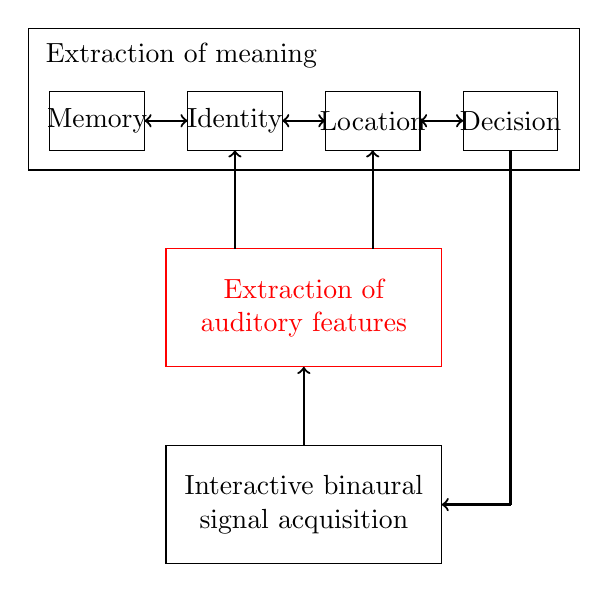
\begin{tikzpicture}
                \draw (-1.75,0) rectangle (1.75,1.5); % binaural simulator
                \node[align=center] at (0,0.75) {Interactive binaural\\ signal acquisition};
                \draw[color=red] (-1.75,2.5) rectangle (1.75,4); % auditory front-end
                \node[align=center,color=red] at (0,3.25) {Extraction of\\ auditory features};
                \draw (-3.5,5) rectangle (3.5,6.8); % blackboard
                \node[right] at (-3.4,6.45) {Extraction of meaning};
                \draw (-3.225,5.25) rectangle (-2.025,6);
                \node at (-2.625,5.625) {\ft Memory};
                \draw (-1.475,5.25) rectangle (-0.275,6);
                \node at (-0.875,5.625) {\ft Identity};
                \draw ( 0.275,5.25) rectangle ( 1.475,6);
                \node at (0.875,5.625) {\ft Location};
                \draw ( 2.025,5.25) rectangle ( 3.225,6);
                \node at (2.625,5.625) {\ft Decision};
                \draw[thick,->] (0,1.5) -- (0,2.5);
                \draw[thick,->] (-0.875,4) -- (-0.875,5.25);
                \draw[thick,->] ( 0.875,4) -- ( 0.875,5.25);
                \draw[thick] (2.625,5.25) -- (2.625,0.75);
                \draw[thick,->] (2.625,0.75) -- (1.75,0.75);
                \draw[thick,<->] (-2.025,5.625) -- (-1.475,5.625);
                \draw[thick,<->] (-0.275,5.625) -- ( 0.275,5.625);
                \draw[thick,<->] ( 1.475,5.625) -- ( 2.025,5.625);
            \end{tikzpicture}
        }
    \end{minipage}
    \hfill
    \begin{minipage}[b]{0.56\columnwidth}

        \centering
        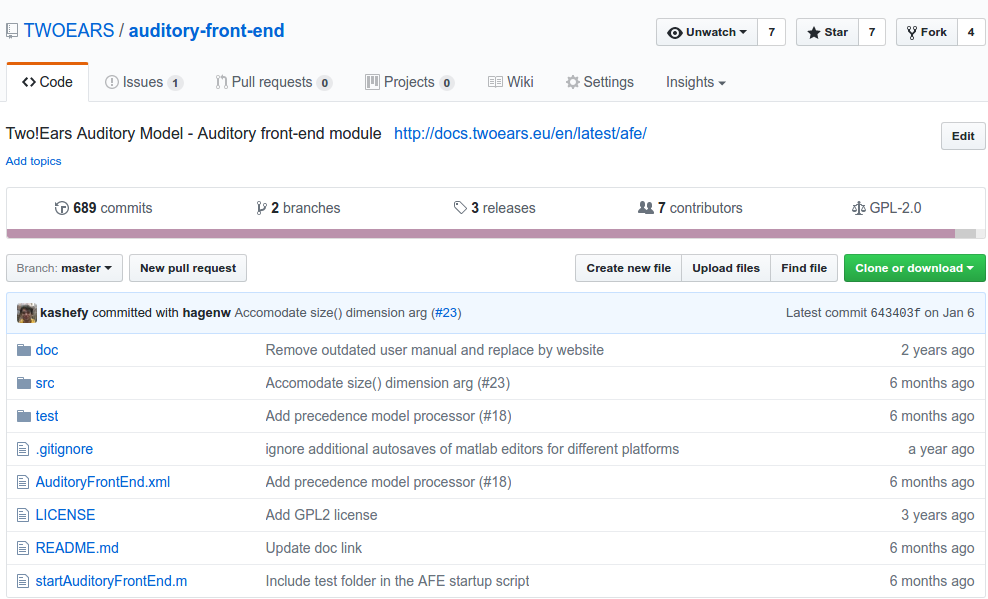
\includegraphics[width=.9\textwidth]{fig/auditory-front-end}

        \begin{itemize}
            \item Standalone ready
            \item Provides auditory features
        \end{itemize}

    \end{minipage}

\end{frame}

%%%%%%%%%%%%%%%%%%%%%%%%%%%%%%%%%%%%%%%%%%%%%%%%%%%%%%%%%%%%%%%%%%%%%%%%%%%%%%%%
\begin{frame}{Two!Ears auditory model}

    \haltpagenumber

    \vspace{1cm}

    \begin{minipage}[b]{0.42\columnwidth}
        \resizebox{\textwidth}{!}{%
            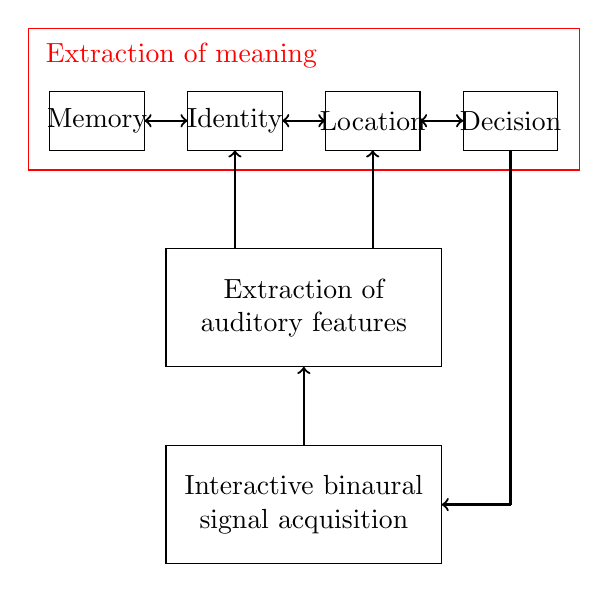
\begin{tikzpicture}
                \draw (-1.75,0) rectangle (1.75,1.5); % binaural simulator
                \node[align=center] at (0,0.75) {Interactive binaural\\ signal acquisition};
                \draw (-1.75,2.5) rectangle (1.75,4); % auditory front-end
                \node[align=center] at (0,3.25) {Extraction of\\ auditory features};
                \draw[color=red] (-3.5,5) rectangle (3.5,6.8); % blackboard
                \node[right,color=red] at (-3.4,6.45) {Extraction of meaning};
                \draw (-3.225,5.25) rectangle (-2.025,6);
                \node at (-2.625,5.625) {\ft Memory};
                \draw (-1.475,5.25) rectangle (-0.275,6);
                \node at (-0.875,5.625) {\ft Identity};
                \draw ( 0.275,5.25) rectangle ( 1.475,6);
                \node at (0.875,5.625) {\ft Location};
                \draw ( 2.025,5.25) rectangle ( 3.225,6);
                \node at (2.625,5.625) {\ft Decision};
                \draw[thick,->] (0,1.5) -- (0,2.5);
                \draw[thick,->] (-0.875,4) -- (-0.875,5.25);
                \draw[thick,->] ( 0.875,4) -- ( 0.875,5.25);
                \draw[thick] (2.625,5.25) -- (2.625,0.75);
                \draw[thick,->] (2.625,0.75) -- (1.75,0.75);
                \draw[thick,<->] (-2.025,5.625) -- (-1.475,5.625);
                \draw[thick,<->] (-0.275,5.625) -- ( 0.275,5.625);
                \draw[thick,<->] ( 1.475,5.625) -- ( 2.025,5.625);
            \end{tikzpicture}
        }
    \end{minipage}
    \hfill
    \begin{minipage}[b]{0.56\columnwidth}

        \centering
        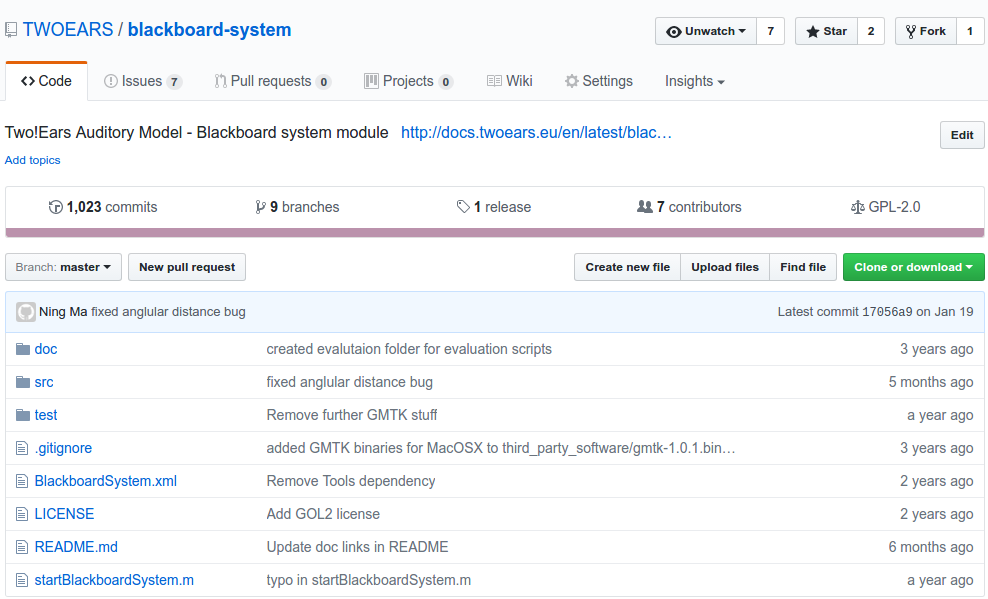
\includegraphics[width=.9\textwidth]{fig/blackboard-system}

        \begin{itemize}
            \item Independent knowledge sources
            \item Needs scheduling
        \end{itemize}

    \end{minipage}

\end{frame}

%%%%%%%%%%%%%%%%%%%%%%%%%%%%%%%%%%%%%%%%%%%%%%%%%%%%%%%%%%%%%%%%%%%%%%%%%%%%%%%%
\begin{frame}{Two!Ears auditory model}

    \haltpagenumber

    \vspace{1cm}

    \begin{minipage}[b]{0.42\columnwidth}
        \resizebox{\textwidth}{!}{%
            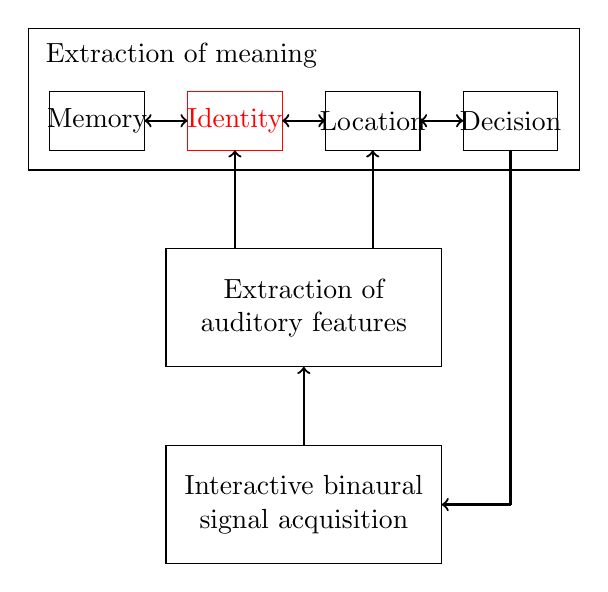
\begin{tikzpicture}
                \draw (-1.75,0) rectangle (1.75,1.5); % binaural simulator
                \node[align=center] at (0,0.75) {Interactive binaural\\ signal acquisition};
                \draw (-1.75,2.5) rectangle (1.75,4); % auditory front-end
                \node[align=center] at (0,3.25) {Extraction of\\ auditory features};
                \draw (-3.5,5) rectangle (3.5,6.8); % blackboard
                \node[right] at (-3.4,6.45) {Extraction of meaning};
                \draw (-3.225,5.25) rectangle (-2.025,6);
                \node at (-2.625,5.625) {\ft Memory};
                \draw[color=red] (-1.475,5.25) rectangle (-0.275,6);
                \node[color=red] at (-0.875,5.625) {\ft Identity};
                \draw ( 0.275,5.25) rectangle ( 1.475,6);
                \node at (0.875,5.625) {\ft Location};
                \draw ( 2.025,5.25) rectangle ( 3.225,6);
                \node at (2.625,5.625) {\ft Decision};
                \draw[thick,->] (0,1.5) -- (0,2.5);
                \draw[thick,->] (-0.875,4) -- (-0.875,5.25);
                \draw[thick,->] ( 0.875,4) -- ( 0.875,5.25);
                \draw[thick] (2.625,5.25) -- (2.625,0.75);
                \draw[thick,->] (2.625,0.75) -- (1.75,0.75);
                \draw[thick,<->] (-2.025,5.625) -- (-1.475,5.625);
                \draw[thick,<->] (-0.275,5.625) -- ( 0.275,5.625);
                \draw[thick,<->] ( 1.475,5.625) -- ( 2.025,5.625);
            \end{tikzpicture}
        }
    \end{minipage}
    \hfill
    \begin{minipage}[b]{0.56\columnwidth}

        \centering
        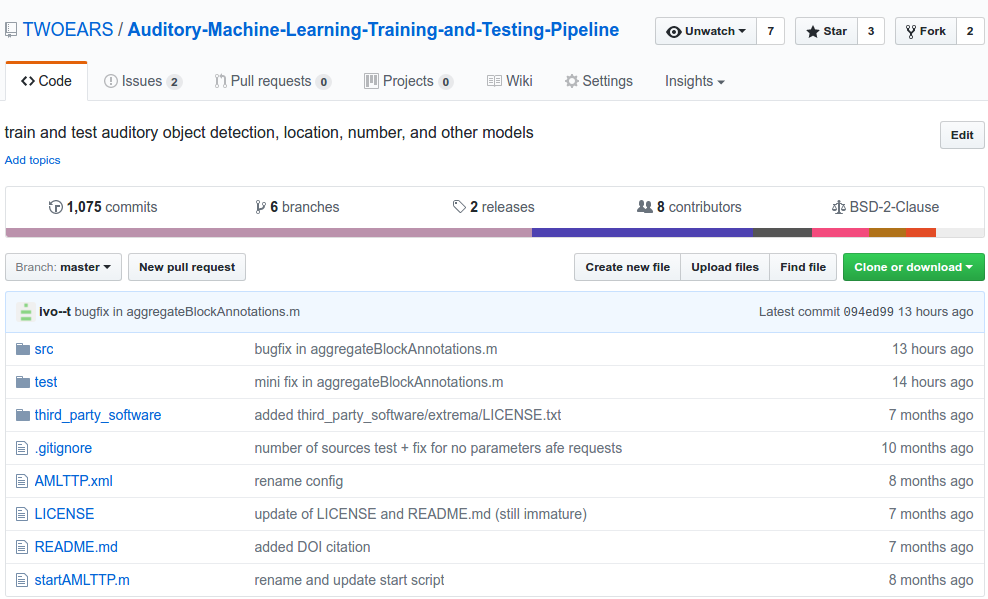
\includegraphics[width=.9\textwidth]{fig/auditory-machine-learning-training}

        \begin{itemize}
            \item Training modules for machine learning
        \end{itemize}

    \end{minipage}

\end{frame}

%%%%%%%%%%%%%%%%%%%%%%%%%%%%%%%%%%%%%%%%%%%%%%%%%%%%%%%%%%%%%%%%%%%%%%%%%%%%%%%%
\begin{frame}{Conclusion on software}

    Things that worked great:
    \begin{itemize}
        \item \href{https://git-scm.com}{git} and
            \href{https://github.com}{github} excellent tools for collaborative
            software development
        \item \href{https://readthedocs.org}{readthedocs} good place for
            creating documentation
    \end{itemize}

    \vspace{0.6cm}

    Proposal for future projects:
    \begin{itemize}
        \item Make a workshop on the topic at the beginning
        \item Include a software engineer for complex software projects
        \item Try to avoid usage of closed-source software (e.g. Matlab)
        \item Introduce how to write reproducible publications
    \end{itemize}

\end{frame}

%%%%%%%%%%%%%%%%%%%%%%%%%%%%%%%%%%%%%%%%%%%%%%%%%%%%%%%%%%%%%%%%%%%%%%%%%%%%%%%%
\begin{frame}{Software depends on data}

    \begin{itemize}
        \item Data is collected and changed during the project:
            \begin{itemize}
                \item HRIR/BRIR measurements for acoustic simulations
                \item Data to train machine learning stages
                \item Listening test results
            \end{itemize}
        \item All partners need access to it
        \item Not all data can be made publicly available
        \item Can have different versions of the same data set
    \end{itemize}

    \vspace{0.5cm}

    $\Rightarrow$ Ideal solution: version control for data + rights management

\end{frame}

%%%%%%%%%%%%%%%%%%%%%%%%%%%%%%%%%%%%%%%%%%%%%%%%%%%%%%%%%%%%%%%%%%%%%%%%%%%%%%%%
\begin{frame}{Possible approaches to data management}

    \begin{itemize}
        \item \href{https://subversion.apache.org}{svn} works, but branching becomes buggy
        \item \href{https://git-scm.com}{git} will produce out of memory errors on your server
            %(as git puts everything in working memory for packing before transmitting it)
            \item \href{https://git-lfs.github.com}{Git Large File Storage} was released during the project, but
            there was no working implementation to set it up on your own server
        \item Similar implementations from the community, like
            \href{https://github.com/alebedev/git-media}{git-media},
            \href{https://git-annex.branchable.com}{git-annex}
        \item Commercial providers like
            \href{http://www.bitkeeper.com/bam.html}{BitKeeper}
    \end{itemize}

\end{frame}

%%%%%%%%%%%%%%%%%%%%%%%%%%%%%%%%%%%%%%%%%%%%%%%%%%%%%%%%%%%%%%%%%%%%%%%%%%%%%%%%
\begin{frame}[fragile]{Our solution to data management}

    \begin{itemize}
        \item Used a \href{https://github.com/TWOEARS/git-media}{modified version
            of git-media} for internal repo \\
        \item Used \href{https://subversion.apache.org}{svn} and
            \href{http://www.redmine.org}{Redmine} for
            \href{https://dev.qu.tu-berlin.de/projects/twoears-getdata/repository}{public
            repo}
        \item In both cases you can download single files and subdirectories
    \end{itemize}

    \vspace{0.8cm}

    \begin{minipage}[t]{.4\columnwidth}
        \centering
        Web-frontend \\
        \vspace{0.2cm}
        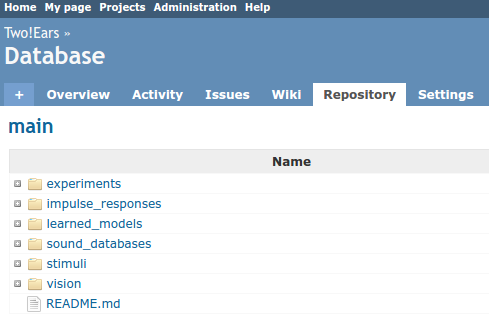
\includegraphics[width=.9\textwidth]{fig/redmine}
    \end{minipage}
    \hfill
    \begin{minipage}[t]{.59\columnwidth}
        \begin{center}
            Matlab interface \\
        \end{center}
        \vspace{0.2cm}
        \small
        \texttt{fname = db.getFile('path/to/file');} \\
        \texttt{sig = audioread(fname);}

        \vspace{1cm}

    \end{minipage}

\end{frame}

%%%%%%%%%%%%%%%%%%%%%%%%%%%%%%%%%%%%%%%%%%%%%%%%%%%%%%%%%%%%%%%%%%%%%%%%%%%%%%%%
\begin{frame}{Conclusion on data management}

    Things that worked ok:
    \begin{itemize}
        \item \href{https://subversion.apache.org}{svn} +
            \href{http://www.redmine.org}{Redmine} for
            \href{https://dev.qu.tu-berlin.de/projects/twoears-getdata/repository}{public
            data}
        \item \href{https://zenodo.org}{zenodo} for releasing single data sets
    \end{itemize}

    \vspace{0.6cm}

    Proposal for future projects:
    \begin{itemize}
        \item Avoid complicated setups (like our git-media)
        \item Hope for better tools
    \end{itemize}

\end{frame}


\end{document}
